% Appendix
\appendix
\section{Appendix}

\subsection{Notation and Symbol Reference}
\label{app:notation}

This section provides a comprehensive reference for all symbols and conventions used throughout this work, following UniTraj framework standards~\cite{unitrajFeng2024} and the \textsc{DatasetItem} type definitions. The following tables have been created using \cite{copilotSonnet}, given the type and shape definitions in \href{https://github.com/JanDuchscherer104/UniTraj/blob/main/unitraj/datasets/types.py}{unitraj/datasets/types.py}.

\begin{table}[H]
\caption{Temporal dimension symbols and definitions}
\centering
\begin{tabular}{p{3cm}p{10cm}}
\toprule
\textbf{Symbol} & \textbf{Definition} \\
\midrule
\(T_p, T_{\text{in}}\) & Number of past timesteps (historical context) \\
\(T_f, T_{\text{out}}\) & Number of future timesteps (prediction horizon) \\
\(T\) & Total trajectory length: \(T = T_p + T_f\) \\
\(\Delta t\) & Temporal sampling interval (i.e.\ 0.1s for 10Hz data) \\
\bottomrule
\end{tabular}
\end{table}

\begin{table}[H]
\caption{Spatial and agent dimension symbols}
\label{tab:shape_symbols}
\centering
\begin{tabular}{p{3cm}p{10cm}}
\toprule
\textbf{Symbol} & \textbf{Definition} \\
\midrule
\(N_{\max}\) & Maximum number of agents in scene (i.e.\ 64) \\
\(N, N_A\) & Actual number of agents in a specific scenario \\
\(N_c\) & Number of center agents, \(N_c = N \) in \cite{lmformerYadav2025}. \\
\(K_{\max}\) & Maximum number of map polylines (i.e.\ 256) \\
\(K\) & Actual number of map polylines in a specific scenario \\
\(L\) & Number of points per map polyline (i.e.\ 20) \\
\( N_L\) & Number of lane segments in \( \boldsymbol{X}_s, N_L=K \cdot L \) \\
\(F_{ap}\) & Agent feature dimension (i.e.\ 39) \\
\(F_{af}\) & Agent future state dimension (4: \(x, y, v_x, v_y\)) \\
\(F_{map}\) & Map feature dimension (i.e.\ 29) \\
\(D\) & Hidden dimension of encodings or latent representations. \\
\bottomrule
\end{tabular}
\end{table}

\begin{table}[H]
\caption{Primary data tensors and their shapes}
\label{tab:data_tensors}
\centering
\begin{tabular}{p{4cm}p{9cm}}
\toprule
\textbf{Tensor} & \textbf{Shape and Description} \\
\midrule
\(\boldsymbol{X}_d\) & \([N_{\max}, T_p, F_{ap}]\) Agent trajectory features \\
\(\boldsymbol{M}_d\) & \([N_{\max}, T_p]\) Agent trajectory validity mask \\
\(\boldsymbol{X}_{d,pos}\) & \([N_{\max}, T_p, 3]\) Agent positions \((x, y, z)\) \\
\(\boldsymbol{X}_{d,last}\) & \([N_{\max}, 3]\) Last observed agent positions \\
\(\tilde{\boldsymbol{X}}_d\) & \([N_{\max}, T_f, F_{af}]\) Agent future states \\
\(\tilde{\boldsymbol{M}}_d\) & \([N_{\max}, T_f]\) Agent future validity mask \\
\(\boldsymbol{y}_c\) & \([T_f, F_{af}]\) Center agent ground truth trajectory \\
\(\boldsymbol{M}_c\) & \([T_f]\) Center agent ground truth validity mask \\
\(\boldsymbol{X}_s\) & \([K_{\max}, L, F_{map}]\) Map polyline features \\
\(\boldsymbol{M}_s\) & \([K_{\max}, L]\) Map polyline validity mask \\
\(\boldsymbol{C}_s\) & \([K_{\max}, 3]\) Map polyline centers \\
\bottomrule
\end{tabular}
\end{table}

Here, \( \tilde{\bullet}_{\circ} \) denotes tensors, expressing future states, while \(\bullet_{\circ}\) denotes tensors for historical or static context. \( \bullet_{d} \) denotes all tensors, representing \emph{dynamic} agents, while \(\bullet_{s}\) denotes tensors for \emph{static} map elements. The center agent, whose trajectory is the target for prediction, is denoted by the subscript \(c\).

\begin{table}[H]
\caption{Agent feature components ($F_{ap} = 39$)}
\centering
\begin{tabular}{p{3cm}p{3cm}p{7cm}}
\toprule
\textbf{Component} & \textbf{Indices} & \textbf{Description} \\
\midrule
Spatial & [0:6] & Position \((x, y, z)\), bbox-dimensions \((l, w, h)\) \\
Type & [6:11] & One-hot agent type encoding as per \ref{tab:agent_types}\\
Temporal & [11:33] & One-hot time embedding (\(T_p + 1\) dimensions) \\
Heading & [33:35] & Heading encoding \((\sin\theta, \cos\theta)\) \\
Kinematic & [35:39] & Velocity \((v_x, v_y)\), acceleration \((a_x, a_y)\) \\
\bottomrule
\end{tabular}
\end{table}

The utilized type encodings are reflecting the respective entity types, which are provided by ScenarioNet~\cite{scenarionetLi2023}, which uses MetaDrive~\cite{metadriveLi2022} internally. It should be noted that the use of these type encodings comes at the loss of more fine-grained semantic annotations that are provided by the original Argoverse2 dataset.

\begin{table}[H]
\caption{Map feature components ($F_{map} = 29$)}
\centering
\begin{tabular}{p{3cm}p{3cm}p{7cm}}
\toprule
\textbf{Component} & \textbf{Indices} & \textbf{Description} \\
\midrule
Position & [0:3] & Current point coordinates \((x, y, z)\) \\
Direction & [3:6] & Direction vector \((d_x, d_y, d_z)\) \\
Previous & [6:9] & Previous point coordinates \((x_{prev}, y_{prev}, z_{prev})\) \\
Lane Type & [9:29] & One-hot lane type encoding (20 categories) \\
\bottomrule
\end{tabular}
\end{table}


\begin{table}[H]
    \caption{Agent type encodings}
    \label{tab:agent_types}
\centering
\begin{tabular}{p{3cm}p{2cm}p{8cm}}
\toprule
\textbf{Type} & \textbf{ID} & \textbf{Description} \\
\midrule
UNSET & 0 & Unknown or unclassified agent \\
VEHICLE & 1 & Cars, trucks, buses, motorcycles \\
PEDESTRIAN & 2 & Pedestrians, wheelchair users \\
CYCLIST & 3 & Bicyclists, e-scooter riders \\
\bottomrule
\end{tabular}
\end{table}

The PolylineType enumeration defines the mapping from MetaDrive/ScenarioNet polyline types to integer labels used in the \(F_{\text{map}}\) feature encoding. This enumeration is derived from the MetaDrive simulation environment~\cite{metadriveLi2022} and ScenarioNet dataset format~\cite{scenarionetLi2023}.

\begin{table}[H]
\centering
\caption{PolylineType Enumeration as per MetaDrive}
\label{tab:polyline-types}
\begin{tabular}{p{2cm}p{11cm}}
\toprule
\textbf{Integer} & \textbf{Description} \\
\midrule
0 & Default/unspecified polyline type \\
1 & Highway or freeway lane \\
2 & Surface street lane \\
3 & Dedicated bicycle lane \\
6 & Broken single white line \\
7 & Solid single white line \\
8 & Solid double white line \\
9 & Broken single yellow line \\
10 & Broken double yellow line \\
11 & Solid single yellow line \\
12 & Solid double yellow line \\
13 & Passing zone double yellow line \\
15 & Road boundary line \\
16 & Median boundary \\
17 & Stop sign location \\
18 & Pedestrian crosswalk \\
19 & Speed bump or traffic calming \\
\bottomrule
\end{tabular}
\end{table}

Note that the conversion from AV2 \( \rightarrow \) ScenarioNet \( \rightarrow \) UniTraj causes many categories to collapse, and plenty of the categories as per \autoref{tab:polyline-types} and  \autoref{tab:agent_types} are actually used, and hence result in degenerate encodings.

\subsection{Deformable Attention}
\label{sec:deformable_attention}

Traditional self and cross-attention in transformers~\cite{vaswani2023attention} scales quadratically with spatial resolution \( \mathcal{O}(H^2W^2) \)\footnote{Note that the sequence consists of \(H \times W\) image patches or activations, and not the original image resolution.}, making it computationally infeasible for high-resolution feature maps. Deformable attention~\cite{zhu2021deformabledetr} addresses this by attending to a sparse set of sampling locations \(\{\mathbf{p}_q + \boldsymbol{\Delta p}_{nqk}\}_{k=1}^{K_s}\) around each query position \(\mathbf{p}_q\), where \(\boldsymbol{\Delta p}_{nqk}\) are dynamically computed \emph{fractional} offsets and \(K_s\) is the number of sampling points per head. This reduces the complexity to \(\mathcal{O}(NHK_s)\)\footnote{Simplified for single head attention}.

For a query with content features \(\mathbf{Z}_q\) with reference point \(\mathbf{p}_q \in [0, 1]^2\) and an input feature map \( \mathbf{X} \) multi-head deformable attention with \( N_h \) heads computes:
\begin{equation}
  \label{eq:deformable_attention_general}
  \text{DeformAttn}(\mathbf{Z}_q, \mathbf{X}, \mathbf{p}_q) = \sum_{n=1}^{N_{H}} \mathbf{W}_n \left[ \sum_{k=1}^{K_s} A_{nkq} \cdot \mathbf{X}(\mathbf{p}_q + \boldsymbol{\Delta p}_{nkq}) \right]
\end{equation}
where \(\mathbf{W}_m\) are learned projection matrices and \(\mathbf{X}(\bullet)\) represents bilinear sampling from the feature map \( \mathbf{X} \in \R^{C \times H \times W} \). Both offsets \(\boldsymbol{\Delta p}_{nkq}\) and attention weights \(A_{nkq}\) are computed via linear projections of the query and key features:
\begin{equation}
\label{eq:deformable_attention_offsets}
\tilde{\bullet} \propto \text{activ}(\underbrace{\mathbf{Z}^T_q \mathbf{U}_n^T}_{\mathbf{Q}}\underbrace{\mathbf{V}_n \mathbf{X}_k}_{\mathbf{K}}) \quad \text{with activ} = \begin{cases}
 &\text{softmax} \text{ for }\tilde{\bullet} = A_{nkq} \\
 &\text{sigmoid} \text{ for }\tilde{\bullet} = \boldsymbol{\Delta p}_{nkq}
\end{cases}
\end{equation}

\( \mathbf{U}_n \) and \( \mathbf{V}_n \) are learned projection matrices to compute the queries \(\mathbf{Q} \) and \emph{keys} \(\mathbf{K}\) in the \( n \)-th attention head. In case of \emph{self}-attention, all the queries, keys, and values are derived from the same sequence, i.e. \( \mathbf{Z}_q = \mathbf{X} \), while in case of \emph{cross}-attention, the queries stem from a different sequence than the keys and values. In a simpler single-head attention setting the keys are computed as \( \mathbf{K} = \mathbf{X}\mathbf{W} \).

\paragraph{Conceptual Interpretation.} To understand deformable attention, it helps to conceptualize the key components~\cite{copilotSonnet}:

\begin{description}[leftmargin=1em,itemsep=3pt]
\item[Queries (\(\mathbf{Q}\)).] Represent \emph{what information is being sought}. In trajectory prediction, queries encode the current prediction state (temporal context and mode embeddings) that determines what spatial features to attend to for generating the next trajectory point.

\item[Keys (\(\mathbf{K}\)) and Values (\(\mathbf{V}\)).] Keys act as \emph{indices} that determine the compatibility between queries and spatial locations, while values contain the \emph{actual feature content} to be aggregated. In CASPFormer, both are derived from the multi-scale CNN feature maps, encoding spatial scene context at different resolutions.

\item[Reference Points (\(\mathbf{p}_q\)).] Serve as \emph{anchor locations} in normalized coordinates \([0,1]^{2}\) that ground the attention mechanism spatially. They represent the current prediction focus (e.g., the last predicted trajectory point) and provide spatial context for where to look in the feature maps.

\item[Sampling Offsets (\(\boldsymbol{\Delta p}_{nkq}\)).] Learned \emph{displacement vectors} that adaptively shift attention away from the reference point toward informative spatial locations. These enable the model to dynamically focus on relevant scene elements (e.g., lane boundaries, nearby agents) rather than being constrained to a fixed grid.

\item[Attention Weights (\(A_{nkq}\)).] Determine the \emph{importance} of each sampled location, allowing the model to emphasize the most relevant spatial features while suppressing irrelevant background information. The weights sum to 1 across all sampling points, creating a normalized spatial attention distribution.
\end{description}

The key innovation is that both offsets and weights are \emph{content-dependent}—computed dynamically based on the current query state rather than being fixed. This enables efficient sparse attention that adapts to the spatial structure of each specific scene, focusing computational resources on the most informative regions.

\subsubsection{Gabor Filter Steerability}
\label{ssec:gabor_filters}
Gabor filters are defined by a sinusoidal plane wave modulated by a Gaussian envelope:
\begin{equation}
\label{eq:gabor_filter}
G_{\lambda,\theta,\psi,\sigma,\gamma}(x,y)
= \exp\!\Bigl(-\tfrac{x'^{2} + \gamma^{2}y'^{2}}{2\sigma^{2}}\Bigr)
  \cos\!\Bigl(2\pi \tfrac{x'}{\lambda} + \psi\Bigr),
\end{equation}
where
\begin{equation}
\label{eq:gabor_rotation}
x' = x\cos\theta + y\sin\theta,\quad
y' = -x\sin\theta + y\cos\theta,
\end{equation}
and \(\lambda\) (wavelength), \(\theta\) (orientation), \(\psi\) (phase), \(\sigma\) (scale), and \(\gamma\) (aspect ratio) control the filter's frequency and spatial extent~\cite{Luan2018GCNN}.

Crucially, Gabor filters are \emph{steerable}, meaning any rotated version can be expressed as a linear combination of a finite set of basis filters:
\begin{equation}
\label{eq:gabor_steerability}
G_{\lambda,\theta}(x,y)
= \sum_{n=1}^N k_n(\theta)\,G_{\lambda,\theta_n}(x,y),
\end{equation}
with fixed prototype orientations \(\{\theta_n\}\) and interpolation coefficients \(\{k_n(\theta)\}\)~\cite{steerableGaborFilters}. This property enables the network to capture directional patterns without having to learn separate filters for each orientation—leading to improved sample efficiency and built-in \(\mathrm{SO}(2)\)-equivariance. In CASPNet, this steerability is leveraged to induce rotational quasi-equivariance in the first layers of the map encoder, ensuring that road elements are represented robustly regardless of global scene orientation. Additionally, by using filter banks that span multiple scales (\(\sigma\)) and aspect ratios (\(\gamma\)), the architecture gains partial \(\mathrm{SIM}(2)\)-equivariance, responding consistently to rescaled and rotated map structures~\cite{steerableGaborFilters}.

%--------------------------------------------------------------------
% \subsection{CASPNet Mathematical Formulations}
% \label{app:caspnet_details}

% \paragraph{Notation.} We denote \(T_p\) and \(T_f\) as the numbers of observed and predicted timesteps, respectively. Following UniTraj conventions~\cite{unitrajFeng2024}, agent trajectories are represented as \(\boldsymbol{X}_d \in \mathbb{R}^{N_{\max} \times T_p \times F_{ap}}\) and map polylines as \(\boldsymbol{X}_s \in \mathbb{R}^{K_{\max} \times L \times F_{map}}\), where \(N_{\max}\) is the maximum number of agents, \(K_{\max}\) is the maximum number of map polylines, \(L\) is the points per polyline, and \(F_{ap}, F_{map}\) are the respective feature dimensions. For rasterized approaches, BEV representations use \(H \times W\) spatial resolution with \(F_d, F_s\) channel dimensions for dynamic and static inputs, respectively.

% \subsubsection{Dual FPN Encoding}
% Rasterized models convert trajectories and HD maps into BEV image stacks:
% \begin{equation}
% \label{eq:app_bev_inputs}
% I_d\in\mathbb{R}^{T_p\times H\times W\times F_d},\quad
% I_s\in\mathbb{R}^{H\times W\times F_s}.
% \end{equation}

% At each level \(\ell\), the trajectory branch produces:
% \begin{equation}
% \label{eq:app_fpn_traj}
% F_{\ell}^{\mathrm{traj}}
% = \mathrm{ConvLSTM}_\ell\Bigl\{\mathrm{CNN}_\ell\bigl(I_d(t)\bigr)\Bigr\}_{t=1}^{T_p},
% \end{equation}
% and the map branch:
% \begin{equation}
% \label{eq:app_fpn_map}
% F_{\ell}^{\mathrm{map}}
% = \mathrm{CNN}_\ell^{\mathrm{Gabor}}(I_s).
% \end{equation}
% These form the multi-scale scene representation:
% \begin{equation}
% \label{eq:app_fpn_fusion}
% \mathcal{F}=\{F_\ell^{\mathrm{traj}}\oplus F_\ell^{\mathrm{map}}\}_{\ell=0}^{L-1}.
% \end{equation}

% \subsection{CASPFormer Mathematical Formulations}
% \label{app:caspformer_details}

% \subsubsection{Deformable Multi-Scale Attention}
% Each query \(q\) attends to \(K\) sampling points across multiple feature levels:
% \begin{equation}
% \label{eq:deformable_sampling}
% p_{q\ell k}=p_q + \Delta p_{q\ell k},
% \end{equation}
% \begin{equation}
% \label{eq:msda}
% \mathrm{MSDA}(Q,K,V) = \sum_{\ell=0}^{L-1}\sum_{k=1}^K A_{q\ell k}\,W_\ell\,V_\ell(p_{q\ell k}),
% \end{equation}
% where \(\Delta p\) are learned sampling offsets and \(A_{q\ell k}\) are attention weights normalized such that \(\sum_{\ell,k} A_{q\ell k} = 1\).

% \subsubsection{Recurrent Cross-Attention Decoder}
% The recurrent decoder maintains:
% \begin{equation}
% \label{eq:dual_query}
% Q_t = T_{t-1} + M,
% \end{equation}
% \begin{equation}
% \label{eq:cross_attention}
% Y_t = \mathrm{CrossDA}(Q_t,Z,r_{t-1}),
% \end{equation}
% with deformable cross-attention defined as:
% \begin{equation}
% \label{eq:crossda_definition}
% \mathrm{CrossDA}(Q,Z,r) = \sum_{\ell,k}A^{\mathit{x}}_{\ell k}\,W_\ell\,Z_\ell(r+\Delta p_{\ell k}).
% \end{equation}

% Outputs \(Y_t\) update both the reference point and temporal queries:
% \begin{equation}
% \label{eq:reference_update}
% r_t = r_{t-1} + \delta_r(Y_t),
% \end{equation}
% \begin{equation}
% \label{eq:temporal_update}
% T_t = \phi(Y_t),
% \end{equation}
% ensuring spatial anchoring around the ego vehicle position and temporal coherence across prediction steps.

% \begin{figure}[ht]
%   \centering
%   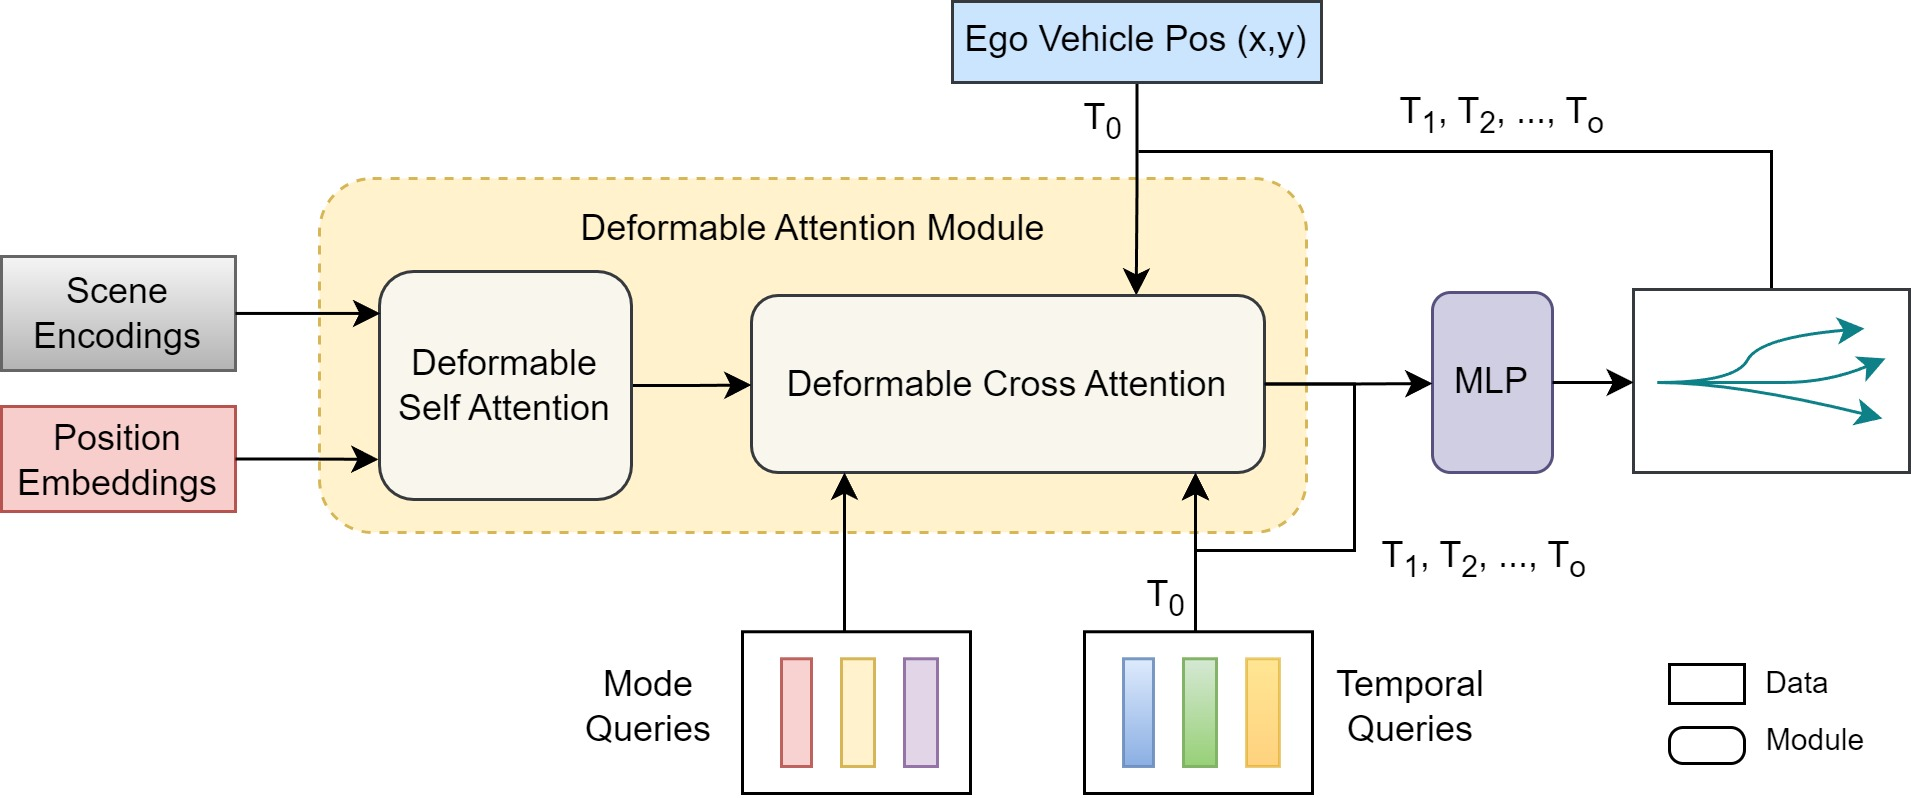
\includegraphics[width=0.8\linewidth]{figures/caspformer_decoder.jpg}
%   \caption{Recurrent deformable cross-attention: updates reference points and temporal queries per step.}
%   \label{fig:recurrent_architecture_appendix}
% \end{figure}

% \subsubsection{Loss Formulation and Multi-Modal Outputs}
% CASPFormer employs a combination of regression and classification losses, following HiVT~\cite{zhou2022hivt}. The approach encourages diversity by optimizing only the best mode, selected based on minimum \(\ell_2\) distance to ground truth:
% \begin{align}
% \label{eq:total_loss}
% \mathcal{L} &= \mathcal{L}_{reg} + \mathcal{L}_{cls}\\
% \label{eq:regression_loss}
% \mathcal{L}_{reg} &= -\frac{1}{T_o} \sum_{t=1}^{T_o} \log[\mathbb{L}(P_t \mid \mu_t, b_t)]\\
% \label{eq:classification_loss}
% \mathcal{L}_{cls} &= -\frac{1}{M} \sum_{k=1}^{M} \log(\pi(k)) \mathbb{L}(P_{T_o,k} \mid \mu_{T_o,k}, b_{T_o,k})
% \end{align}
% where \(\mathbb{L}\) denotes the Laplacian distribution, \(\mu_t\) and \(b_t\) are position and uncertainty of the best mode, \(P_t\) are ground truth positions, and \(\pi(k)\) are mode probabilities.

% A shared MLP decodes \(Y_t\) to \(\{\mu_{t,k},\pi_{t,k}\}_{k=1}^M\), modeling a mixture distribution over predicted modes:
% \begin{equation}
% \label{eq:mixture_distribution}
% \mathcal{P}(\boldsymbol{\mu}_t, b_t) = \sum_{k=1}^{M} \pi_k \cdot \mathbb{L}(\boldsymbol{\mu}_t \mid \boldsymbol{\mu}_{t,k}, b_{t,k})
% \end{equation}

%--------------------------------------------------------------------

\subsection{The UniTraj Dataprocessing Pipeline}
\label{app:framework}

\textbf{Phase 1: Temporal Window Extraction}
The first processing stage extracts \emph{uniformly sampled} windows containing historical context (\(T_p\) steps) and future ground truth (\(T_f\) steps) from raw agent trajectories. Frequency masking ensures consistent uniform temporal resolution with a sampling interval \(\Delta t_{s}\) across datasets, and is combined with the original validity masks to indicate which observations are valid at each timestep. Validity masks indicate missing observations throughout the pipeline.

\begin{algorithm}[H]
\caption{Phase 1: Temporal Window Extraction}
\label{alg:phase1_temporal}
\begin{algorithmic}[1]
\REQUIRE Raw scenario tracks \(\mathcal{T}\), time horizons \(T_p, T_f\), sampling interval \(\Delta t_{s}\)
\ENSURE Temporally windowed agent trajectories with validity masks
\STATE \(T_{total} \leftarrow T_p + T_f\) \COMMENT{Total time window length}
\STATE \(M_{freq} \leftarrow \text{generate\_mask}(T_p - 1, T_{total}, \Delta t_{s})\) \COMMENT{Temporal sampling mask}
\FOR{each agent track \(i \in \mathcal{T}\), timestep \(t = 0\) to \(T_{total}\)}
    \STATE Extract state vectors: \(\boldsymbol{s}_i^{(t)} = [\boldsymbol{p}_i^{(t)}, l_i, w_i, h_i, \theta_i^{(t)}, \boldsymbol{v}_i^{(t)}, \text{valid}_i^{(t)}]^T\)
    \STATE Apply temporal windowing: \(\boldsymbol{s}_i \leftarrow \boldsymbol{s}_i[t_{start} : t_{start} + T_{total}]\)
    \STATE Apply frequency masking: \(\text{valid}_i^{(t)} \leftarrow \text{valid}_i^{(t)} \cdot M_{freq}[t]\)
\ENDFOR
\end{algorithmic}
\end{algorithm}

\textbf{Phase 2: Map Feature Processing}

This phase converts heterogeneous map primitives (lanes, boundaries, signs, crosswalks) into standardized polyline sequences with consistent geometric and semantic encoding. Polyline interpolation ensures uniform point density, direction vectors encode the local orientation of each segment, and type-based filtering selects relevant map elements for prediction scenarios.

\begin{algorithm}[H]
\caption{Phase 2: Map Feature Processing}
\label{alg:phase2_map}
\begin{algorithmic}[1]
\REQUIRE Raw map data \(\mathcal{M}\), interpolation distance \(d_{interp}\)
\ENSURE Standardized map polylines with geometric and semantic features
\FOR{each map element \(m \in \mathcal{M}\)}
    \STATE Interpolate polyline points with uniform spacing \(d_{interp}\)
    \STATE Compute direction vectors: \(\boldsymbol{d}_{k,l} = \boldsymbol{p}_{k,l+1} - \boldsymbol{p}_{k,l}\)
    \STATE Assign semantic type encoding: \(\boldsymbol{o}_{type} \in \{0,1\}^{20}\)
    \STATE Store polyline: \(\boldsymbol{L}_k = [\boldsymbol{p}_{k,l}, \boldsymbol{d}_{k,l}, \boldsymbol{o}_{type}]_{l=1}^{L}\)
\ENDFOR
\end{algorithmic}
\end{algorithm}

\textbf{Phase 3: Agent Selection and Filtering}

Agent filtering ensures that only relevant trajectories with sufficient motion and observation quality are retained for training. This phase applies distance-based motion thresholds, present-time validity requirements, and future continuity constraints to identify suitable center agents.

\begin{algorithm}[H]
\caption{Phase 3: Agent Selection and Filtering}
\label{alg:phase3_filtering}
\begin{algorithmic}[1]
\REQUIRE Agent trajectories \(\mathcal{A}\), motion threshold \(d_{min} = 2.0\)m
\ENSURE Filtered set of center agents \(\mathcal{A}_{center}\)
\STATE \(\mathcal{A}_{center} \leftarrow \emptyset\)
\FOR{each agent \(i \in \mathcal{A}\)}
    \STATE Compute total motion: \(\Delta d_i = \sum_{t=1}^{T_p-1} \|\boldsymbol{p}_i^{(t)} - \boldsymbol{p}_i^{(t-1)}\|_2\)
    \IF{\(\Delta d_i \geq d_{min}\) AND \(\text{valid}_i^{(T_p-1)} = 1\)}
        \STATE Add to center agents: \(\mathcal{A}_{center} \leftarrow \mathcal{A}_{center} \cup \{i\}\)
    \ENDIF
\ENDFOR
\end{algorithmic}
\end{algorithm}

\textbf{Phase 4: Coordinate System Transformation}

For each center agent, the entire scene (including all other agents and map elements) is transformed to an agent-centric coordinate frame. This transformation consists of translation to center the agent's position at \(t = T_p - 1\) at the origin, followed by rotation to align the agent's heading with the positive \(x\)-axis.

\begin{algorithm}[H]
\caption{Phase 4: Coordinate System Transformation}
\label{alg:phase4_transform}
\begin{algorithmic}[1]
\REQUIRE Center agent \(c\), all trajectories \(\mathcal{A}\), map polylines \(\mathcal{L}\)
\ENSURE Agent-centric coordinates for all elements
\STATE \(\boldsymbol{p}_c^{ref} \leftarrow \boldsymbol{p}_c^{(T_p-1)}\) \COMMENT{Reference position}
\STATE \(\theta_c^{ref} \leftarrow \theta_c^{(T_p-1)}\) \COMMENT{Reference heading}
\FOR{each agent \(i \in \mathcal{A}\), timestep \(t\)}
    \STATE Translate: \(\boldsymbol{p}_i^{(t)} \leftarrow \boldsymbol{p}_i^{(t)} - \boldsymbol{p}_c^{ref}\)
    \STATE Rotate: \(\boldsymbol{p}_i^{(t)} \leftarrow \mathbf{R}(-\theta_c^{ref}) \boldsymbol{p}_i^{(t)}\)
    \STATE Transform heading: \(\theta_i^{(t)} \leftarrow \theta_i^{(t)} - \theta_c^{ref}\)
    \STATE Rotate velocity: \(\boldsymbol{v}_i^{(t)} \leftarrow \mathbf{R}(-\theta_c^{ref}) \boldsymbol{v}_i^{(t)}\)
\ENDFOR
\FOR{each polyline \(k \in \mathcal{L}\), point \(l\)}
    \STATE Apply same coordinate transformation to polyline points
    \STATE Filter polylines within spatial range: \(\|\boldsymbol{p}_{polyline}\|_2 \leq \text{map\_range}\)
\ENDFOR
\end{algorithmic}
\end{algorithm}

After this transformation, all spatial map features and agent states are expressed in a common reference frame, whose origin is the center agent's position at the last historical timestep \(T_p-1\). This yields both \emph{translation} and \emph{rotation} invariance, when perceiving the scene from the center agent's perspective.

\textbf{Phase 5: Feature Vector Assembly}

This phase constructs the full feature vectors for each agent by concatenating spatial state, agent type encoding, temporal step embedding, heading representation, and kinematic features. Invalid trajectory points are zeroed out according to the validity masks.

\begin{algorithm}[H]
\caption{Phase 5: Feature Vector Assembly}
\label{alg:phase5_features}
\begin{algorithmic}[1]
\REQUIRE Transformed agent states, validity masks
\ENSURE Complete agent feature vectors \(\boldsymbol{X}_d \in \mathbb{R}^{N_{\max} \times T_p \times F_{ap}}\)
\FOR{each agent \(i\), timestep \(t\)}
    \STATE Spatial features: \(\boldsymbol{f}_{spatial} = [\boldsymbol{p}_i^{(t)}, l_i, w_i, h_i] \in \mathbb{R}^6\)
    \STATE Type encoding: \(\boldsymbol{o}_{type} \in \{0,1\}^5\)
    \STATE Time embedding: \(\boldsymbol{e}_{time} \in \{0,1\}^{T_p+1}\)
    \STATE Heading encoding: \(\boldsymbol{h}_{embed} = [\sin(\theta_i^{(t)}), \cos(\theta_i^{(t)})] \in \mathbb{R}^2\)
    \STATE Kinematic features: \(\boldsymbol{f}_{kinematic} = [\boldsymbol{v}_i^{(t)}, \boldsymbol{a}_i^{(t)}] \in \mathbb{R}^4\)
    \STATE Concatenate: \(\boldsymbol{X}_d^{(i,t)} = [\boldsymbol{f}_{spatial}, \boldsymbol{o}_{type}, \boldsymbol{e}_{time}, \boldsymbol{h}_{embed}, \boldsymbol{f}_{kinematic}]\)
    \IF{\(\text{valid}_i^{(t)} = 0\)}
        \STATE \(\boldsymbol{X}_d^{(i,t)} \leftarrow \boldsymbol{0}\)
    \ENDIF
\ENDFOR
\end{algorithmic}
\end{algorithm}

\textbf{Phase 6: Agent Proximity Filtering and Padding}

To ensure computational tractability, the pipeline retains only the \(N_{\max}\) closest agents to each center agent, where proximity is measured by the Euclidean distance at the final historical timestep. Agent features are then zero-padded to the fixed dimension \(N_{\max}\) to enable efficient batch processing.

\begin{algorithm}[H]
\caption{Phase 6: Agent Proximity Filtering and Padding}
\label{alg:phase6_proximity}
\begin{algorithmic}[1]
\REQUIRE Agent features \(\boldsymbol{X}_d\), maximum agents \(N_{\max} = 64\)
\ENSURE Padded agent tensor \(\boldsymbol{X}_d \in \mathbb{R}^{N_{\max} \times T_p \times F_{ap}}\)
\FOR{each center agent \(c\)}
    \STATE Compute distances: \(d_{ic} = \|\boldsymbol{p}_i^{(T_p-1)} - \boldsymbol{p}_c^{(T_p-1)}\|_2\) for all agents \(i\)
    \STATE Select top-\(N_{\max}\) closest agents by distance
    \STATE Zero-pad features to dimension \(N_{\max} \times T_p \times F_{ap}\)
    \STATE Create validity mask: \(\boldsymbol{M}_d \in \{0,1\}^{N_{\max} \times T_p}\)
\ENDFOR
\end{algorithmic}
\end{algorithm}

\textbf{Phase 7: Map Feature Processing}

The agent-centric map polylines are converted into a fixed-size tensor representations in a three-stage process: segmentation based on geometric discontinuities (gaps \(>\) 1.0m), uniform resampling to exactly \(L\) points per segment, and proximity-based selection of the top \(K_{\max}\) segments closest to the center agent. Each point is encoded with geometric context including position, direction vectors, previous point reference, and semantic type information. The resulting map tensor \(\boldsymbol{X}_s\) is padded to a fixed size of \(K_{\max}\) segments, each with \(L\) points, and a validity mask \(\boldsymbol{M}_s\) is created to indicate which segments are actually present.

\begin{algorithm}[H]
\caption{Phase 7: Map Feature Processing}
\label{alg:phase7_map_features}
\begin{algorithmic}[1]
\REQUIRE Agent-centric polylines, max polylines \(K_{\max} = 256\), points per polyline \(L = 20\)
\ENSURE Map tensor \(\boldsymbol{X}_s \in \mathbb{R}^{K_{\max} \times L \times F_{map}}\), validity mask \(\boldsymbol{M}_s\)
\FOR{each polyline \(k\)}
    \STATE Segment polyline at geometric discontinuities (gaps \(> 1.0\)m)
    \STATE Resample each segment to exactly \(L\) uniform points
    \STATE Compute geometric features: position, direction, previous point
    \STATE Append semantic type encoding: \(\boldsymbol{o}_{type} \in \{0,1\}^{20}\)
    \STATE Assemble: \(\boldsymbol{X}_s^{(k,l)} = [\text{position}, \text{direction}, \text{previous}, \boldsymbol{o}_{type}]\)
\ENDFOR
\STATE Select top-\(K_{\max}\) polylines by proximity to center agent
\STATE Zero-pad to fixed dimensions and create validity mask
\end{algorithmic}
\end{algorithm}

\textbf{Phase 8: Future Trajectory Processing}

This phase processes the future trajectory ground truth for each agent and creates the center agent's target trajectory. Future trajectories are extracted, transformed to agent-centric coordinates, and validity masks are created to handle variable-length future observations.

\begin{algorithm}[H]
\caption{Phase 8: Future Trajectory Processing}
\label{alg:phase8_future}
\begin{algorithmic}[1]
\REQUIRE Future trajectory data, center agent indices
\ENSURE Center ground truth \(\boldsymbol{y}_c \in \mathbb{R}^{T_f \times 4}\), validity masks
\FOR{each agent \(i\), future timestep \(t \in [T_p, T_p + T_f)\)}
    \STATE Extract future state: \(\boldsymbol{s}_i^{(t)} = [\boldsymbol{p}_i^{(t)}, \boldsymbol{v}_i^{(t)}]\)
    \STATE Apply agent-centric transformation
    \STATE Store in future tensor: \(\tilde{\boldsymbol{X}}_d[i, t-T_p] = \boldsymbol{s}_i^{(t)}\)
\ENDFOR
\FOR{each center agent \(c\)}
    \STATE Extract center ground truth: \(\boldsymbol{y}_c = \tilde{\boldsymbol{X}}_d[c, :, :]\)
    \STATE Create future validity mask: \(\tilde{\boldsymbol{M}}_d \in \{0,1\}^{T_f}\)
    \STATE Compute final valid index: \(idx_{final} = \max\{t : \tilde{\boldsymbol{M}}_d[t] = 1\}\)
\ENDFOR
\end{algorithmic}
\end{algorithm}

\textbf{Phase 9: DatasetItem Assembly}

The final processing phase assembles all processed components into final \texttt{DatasetItem} instances. It performs data validation, applies optional attribute masking (e.g., zeroing z-coordinates or object bounding boxes), ensures float32 compatibility, and finally creates structured \texttt{DatasetItem} instances.
\begin{algorithm}[H]
\caption{Phase 9: DatasetItem Assembly}
\label{alg:phase9_assembly}
\begin{algorithmic}[1]
\REQUIRE All processed tensors and masks
\ENSURE Final \texttt{DatasetItem} instance
\STATE Create \texttt{DatasetItem} instance with all processed tensors
\STATE Apply attribute masking (optional): zero out z-axis, size, velocity, etc.
\STATE Convert floating data types to float32
\RETURN \texttt{DatasetItem} instance
\end{algorithmic}
\end{algorithm}

The resulting \texttt{DatasetItem}'s are subsequently saved to disk for training and evaluation. They include all agent tensors, map tensors, ground truth labels, and validity masks as \texttt{numpy} arrays in various formats for easy handling at different training, evaluation or visualization stages.
